\chapter{SLAM Framework}
\label{chapter:ScaViSLAM}

This chapter will describe the underlying SLAM system used for this work, ScaViSLAM.  ScaViSLAM, (Scalable Visual SLAM) is a stereo visual SLAM algorithm designed to do online constant time SLAM. It achieves this by using a SLAM graph, and instead of optimizaing over the whole graph, it optimizes using a 'double window' approach to select which parts of the graph to optimize.  It consists an in 'inner window', where a bundle adjustment over all poses and landmarks is performed, and an outer window, where an optimization over only keyframes and keyframe-keyframe edges is done. The outer and inner window are dynamically calculated by the algorithm during operation.  This double-window approach allows for only a subsection of the graph to be optimized each step, thus solving in constant time, whilst still allowing for the entire graph to remain consistent.

The inner workings of ScaViSLAM may be broken up into three different modules, each of which runs in a seperate thread; the stereo frontend, SLAM graph backend and place recognition. These modules will be discussed here. In addition to the modules, the operation of the SLAM graph will be expanded on, as not only is this the main novelty of the ScaViSLAM algorithm, but is also very important in the context of the contribution of this work. The main interface between the algorithm presented in this work and ScaViSLAM system is by adding information to the SLAM graph.

\section{Frontend}
\label{sec:scavislam_frontend}

The frontend is responsible for calculating visual odometry.  It also finds landmarks and estimates their 3D positions using stereo information.  It is also responsible for creating new keyframes, containing all the logic for when to generate a new keyframe or switch to an old one. 

\subsection{Visual Odometry}

%TODO: brief/fast citation

To calculate an initial transformation between frames, first a disparity image is calculated using dense stereo matching, then dense stereo tracking is performed.  Both of these operations are done on the GPU.  After an initial transformation has been estimated, landmarks are matched used guided BRIEF (citation) at FAST (citation) corners locations.  Matching is done on multiple image pyramid levels to enable some degree of scale invariance. Selection of landmarks will be discussed in the following section.  Image patches of landmarks are warped into the current perspective by using the current transformation to improve matching. Having matched enough points against current and previous keyframes, a refined pose is calculated by minimising reprojection error of all point correspondences.

\subsection{Tracking points}

In an outdoor setting there are often many landmarks to track and therefore it is important to select reliable points to track in the interest of robustness and scalability.  Therefore the following criteria is applied:
\begin{itemize}
 \setlength{\itemsep}{0cm}%
 \setlength{\parskip}{0cm}%
 \item Visible from either current keyframe or adjacent keyframe
 \item Reprojection error is within a threshold
 \item Not too far
 \item Not too close
 \item Change in viewing angle between frames not too large
\end{itemize}

\subsection{Creates Keyframes}

New keyframes are added either when the number of shared observations drops below a certain threshold, or a certain metric distance from the last keyframe has been passed.  This ensures good interconnectivity between all keyframes.  As new keyframes, landmarks and landmark observations are created, these are passed to the backend to be integrated into the graph.

\section{Backend}
\label{sec:scavislam_backend}

The backend is responsible for maintaining the entire SLAM graph, and thus holds internally its own representation of the whole graph.  It provides interfaces for other modules to add information to the graph. It also acts as a wrapper for the graph solving library, in this case g2o. As the graph is designed to run in constant time, the backend has been designed to execute at a relatively fast rate (insert number here) so that the graph may be constantly solved during operation.
%TODO: determine backend speed

%\subsection{Contains the entire graph (not in g2o format)}
%\subsection{Performs some bundle adjustment}
%\subsection{Acts as a wrapper for g2o}

The backend also serves as a wrapper for the graph optimizer.  It contains data structures to represent all keyframes, keyframe edges, landmarks and landmark observations.  For each optimization, only the necessary keyframes and edges are copied into the optimizer.  After optimization has been performed, the optimized vertices are copied back to ScaViSLAM representation of the graph, and the optimizer object is discarded.

\section{Place Recognition}
\label{sec:scavislam_place_recog}

The place recognition module is responsible for detecting 'large loop closures' between keyframes.
(see section \ref{subsec:loop_closure}).

\subsection{Bag of words}

One solution to finding large loop closures between keyframes would be to compare every keyframe with every other keyframe generated.  However this would result in a time complexity of $O(n^2)$ for n frames.  This does clearly not scale to large maps.

A better solution is to use a place recognition algorithm, which given a collection of images of various locations, attempts to match a query frame to an existing location, or say if the frame is a completely new location without searching through the entire image space.  There has been considerable research in place recognition in recent times (cite a bunch of papers).  In ScaViSLAM the bag of words approach was employed.

%TODO: read about bag of words and summarize

The current implementation of bag of words returns a score for every frame (check this).  If the score is above a certain threshold, this frame pair will be identified as a potential loop closure and then tested with a geometry check.

\subsection{Geometry check}

The geometry check serves two purposes; one is to filter out false positives as generated by the place recognition module.  The bag of words implementation in ScaViSLAM is rather simplistic and as a result outputs many false positives.  The second purpose is to generate an estimation of the pose between keyframes so it may be integrated into the SLAM graph.  

To do this check, features are extracted from both frames and projected to 3D points using stereo information.  3D-3D correspondences are obtained from feature matching between frames and RANSAC is used to find an optimal transformation.  If enough inliers are returned then the edge may be added to the graph.  The number of inliers may be used to weight the strength of this pose-pose graph constraint.

\subsection{Readjustment of double window}
%TODO: move this section to double window
Due to the double window approach, simply adding the pose constraint will not close the loop, as pose edges are not considered in the inner window.  Instead, the current keyframe is initialized to its new position based on the loop closure edge, and then shared observations between current and old keyframes are searched for.  If successful, The landmarks are merged and the old keyframes are added to the inner window.  Optimization is then executed with the new double window.  The inner window pulls old and new keyframes together, while the outer window propagates error throughout the rest of the graph.

\section{ScaViSLAM Graph}
\label{sec:scavislam_graph}

\subsection{g2o}

g2o is c++ framework for solving optimization of non-linear least squares problems that can be described by a hyper-graph. A hyper-graph is an extension of a graph where an edge can connect two or more nodes together. 

To express an optimization problem as a graph, one can think of vertices as being variables, or states, to optimize over, and edges as being constraints for 1 or more vertices.  Edges for a single vertex are called unary edges, for two vertices binary edges and more than 2 multi edges.  Vertex states may be one or more dimensions.  Having said that, vertices may also be used as parameters in the optimization problem.  Error functions to minimise are then defined as how well vertex states fit their edge constraints.

An example of how a simple SLAM problem may be expressed as a hyper-graph is shown below.
\begin{figure}[h]
  \centering
      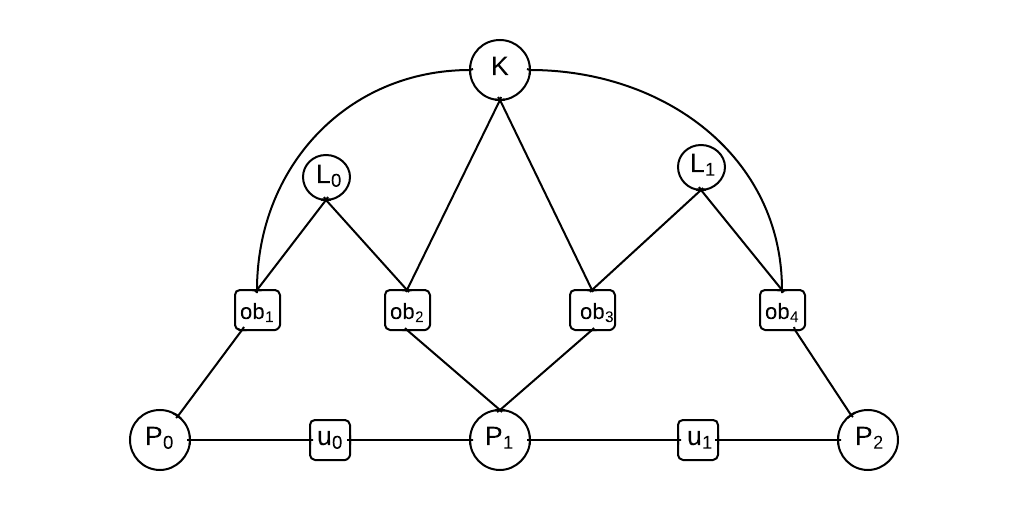
\includegraphics[width=1.0\textwidth]{chapters/images/simple_slam}
  \caption{A simple SLAM graph for a generic robot.  Circles are vertices to optimize over, and
squares are edges, which in this case are measurements}
\end{figure}

The diagram shows robot poses as $\bv P_i$.  These poses could be represented by any number of dimensions. In the case of an exploratory robot, this is likely to be 3 dimensional (x, y, and yaw for movement on a fixed plane), or 6 dimensional (x, y, z, rotation about x, rotation about y, rotation about z).  $\bv U_i$ are binary edges, representing odometry measurements between robot poses. These are measurements or constraints and will remain unchanged during optimization.  $\bv L_i$ represents unique landmarks that the robot can sense and make some form of measurement relative to its own position, as well as re-identify in different robot poses.  A landmark could be a corner from a laser scan or a feature point in a camera image.  K represents calibration parameters of the sensor.  This could be something like an offset, camera intrinsic parameters, or an extrinsic parameter to transform the sensor readings from the sensor frame to the robot frame.  $\bv {ob}_i$ are observation multi-edges, between a robot pose, a landmark, and the calibration parameter.

Such an example of graph optimization would allow an optimization of the poses of the robot, positions of the landmarks, and the sensor calibration, based on all odometry and observation measurements.

In order to compute this optimization, the generic graph problem may be represented mathematically as follows:

 \begin{align}
   \bv{F}(\bv x) &= \sum\limits_{K \in C}^{} 
                 \bv e_k(\bv x_k, \bv z_k)^T 
                 \bv \Omega_k
                 \bv e_k(\bv x_k, \bv z_k)  \\ 
   \bv x^* &= \operatornamewithlimits{argmin}\limits_{\bv x}\bv{F}(\bv x)
 \end{align}

\begin{itemize}
 \item $\bv x$ is a vector of parameter sets, whereby each $\bv x_i$ is a parameter block
 \item $\bv x_k$ is a set of parameters involved in the $k$th constraint
 \item $\bv z_k$ is a constraint or measurement relating to parameter $\bv x_k$
 \item $\bv \Omega_k$ is the information matrix for $\bv z_k$.  This can be used to weight this constraint
 \item $\bv e_k(\bv x_k, \bv z_k)$ is the error function that measures how well parameter block $\bv x_k$ satisfies $\bv z_k$.  If for instance $\bv z_k$ directly measured $\bv x_k$, then a straightforward error function would be $\bv e_k(\bv x_k, \bv z_k) = \bv x_k - \bv z_k $
\end{itemize}

\subsubsection{Solving the Least squares problem}

%TODO: citations
A numerical solution to eq. 4.2 can be performed using a non linear solver such as Gauss-Newton or Levenberg-Marquardt (cite, cite).  The error function can be approximated by its first order Taylor expansion around the current initial guess $\breve{\bv x}$

\begin{align}
  \bv e_k(\breve{\bv x}_k + \Delta \bv x_k) &= \bv e_k(\breve{\bv x} + \Delta \bv x) \\
      & \simeq \bv e_k + \bv J_k \Delta \bv x
\end{align}

$\bv J_k$ is the Jacobian of $\bv e_k(\bv x)$ computed in $\breve{\bv x}$.  Substituting eq(4.4) as the error function in eq(4.1), one obtains:

\begin{align}
  \bv F(\breve{\bv x} + \Delta \bv x) &= \bv e_k(\breve{\bv x} + \Delta \bv x)^T \bv \Omega_k \bv e_k(\breve{\bv x} + \Delta \bv x) \\
  & \simeq (\bv e_k + \bv J_k \Delta \bv x)^T 
    \bv \Omega_k 
    (\bv e_k + \bv J_k \Delta \bv x) \\
  &= \bv e_k^T \bv \Omega_k \bv e_k 
    + 2 \bv e_k^T \bv \Omega_k \bv J_k \Delta \bv x 
    + \Delta \bv x^T \bv J_k^T \bv \Omega_k \bv J_k \Delta \bv x \\
  &= c_k + 2\bv b_k \Delta \bv x + \Delta \bv x \bv H_k \Delta \bv x
\end{align}

Where $c_k = \bv e_k^T \bv \Omega_k \bv e_k$, $\bv b_k = \bv e_k^T \bv \Omega_k \bv J_k$ and $\bv H_k = \bv J_k^T \bv \Omega_k \bv J_k$. This quadratic form can then be minimized in $\Delta \bv x$ by solving the linear system

\begin{align}
   \bv H \Delta \bv x^* = -\bv b
\end{align}

$\bv H$ is a very large sparse square matrix.  It is mostly zeros; it only contains non zero values where there is a constraint connecting blocks.  This matrix can be efficiently solved by taking advantage of the fact that is is sparse, for instance, by Cholesky factorization.

\subsubsection{Error functions}
%TODO: error fn fill in 
This would talk about how to design the error function.  Talk about for instance how to turn an SE(3) into a 6D vector.  Lie algebra will be mentioned for SE(3) edge case. 

\subsubsection{Operator to apply increments in Optimization}
%TODO: oplus fill in 
Non Euclidean nature of parameters.  For instance rotations are not Euclidean.  Define a $\boxplus$ operator to add an increment to the vertex states.  For instance take vector part of Quaternion or use some Lie algebra whatever. explain SE(3) example 

\subsubsection{Robust least squares}
%TODO huber fill in or remove
Use huber instead of squares to make robust against outliers.  Mention that g2o can define this per edge.  Do a figure of the function!

\subsection{Graph description}

Having discussed the graph solver used by this package, the specific SLAM graph implementation will be covered here.  The graph may be split up into two parts, an inner and an outer window.  These will be described first separately, and following how they work together.

\subsubsection{Inner Window}

The inner window is a bundle adjustment over poses of the camera, as well as landmark positions, using edges of landmark observations.  See fig \ref{fig:inner_window}.

\begin{figure}[h!]
  \centering
    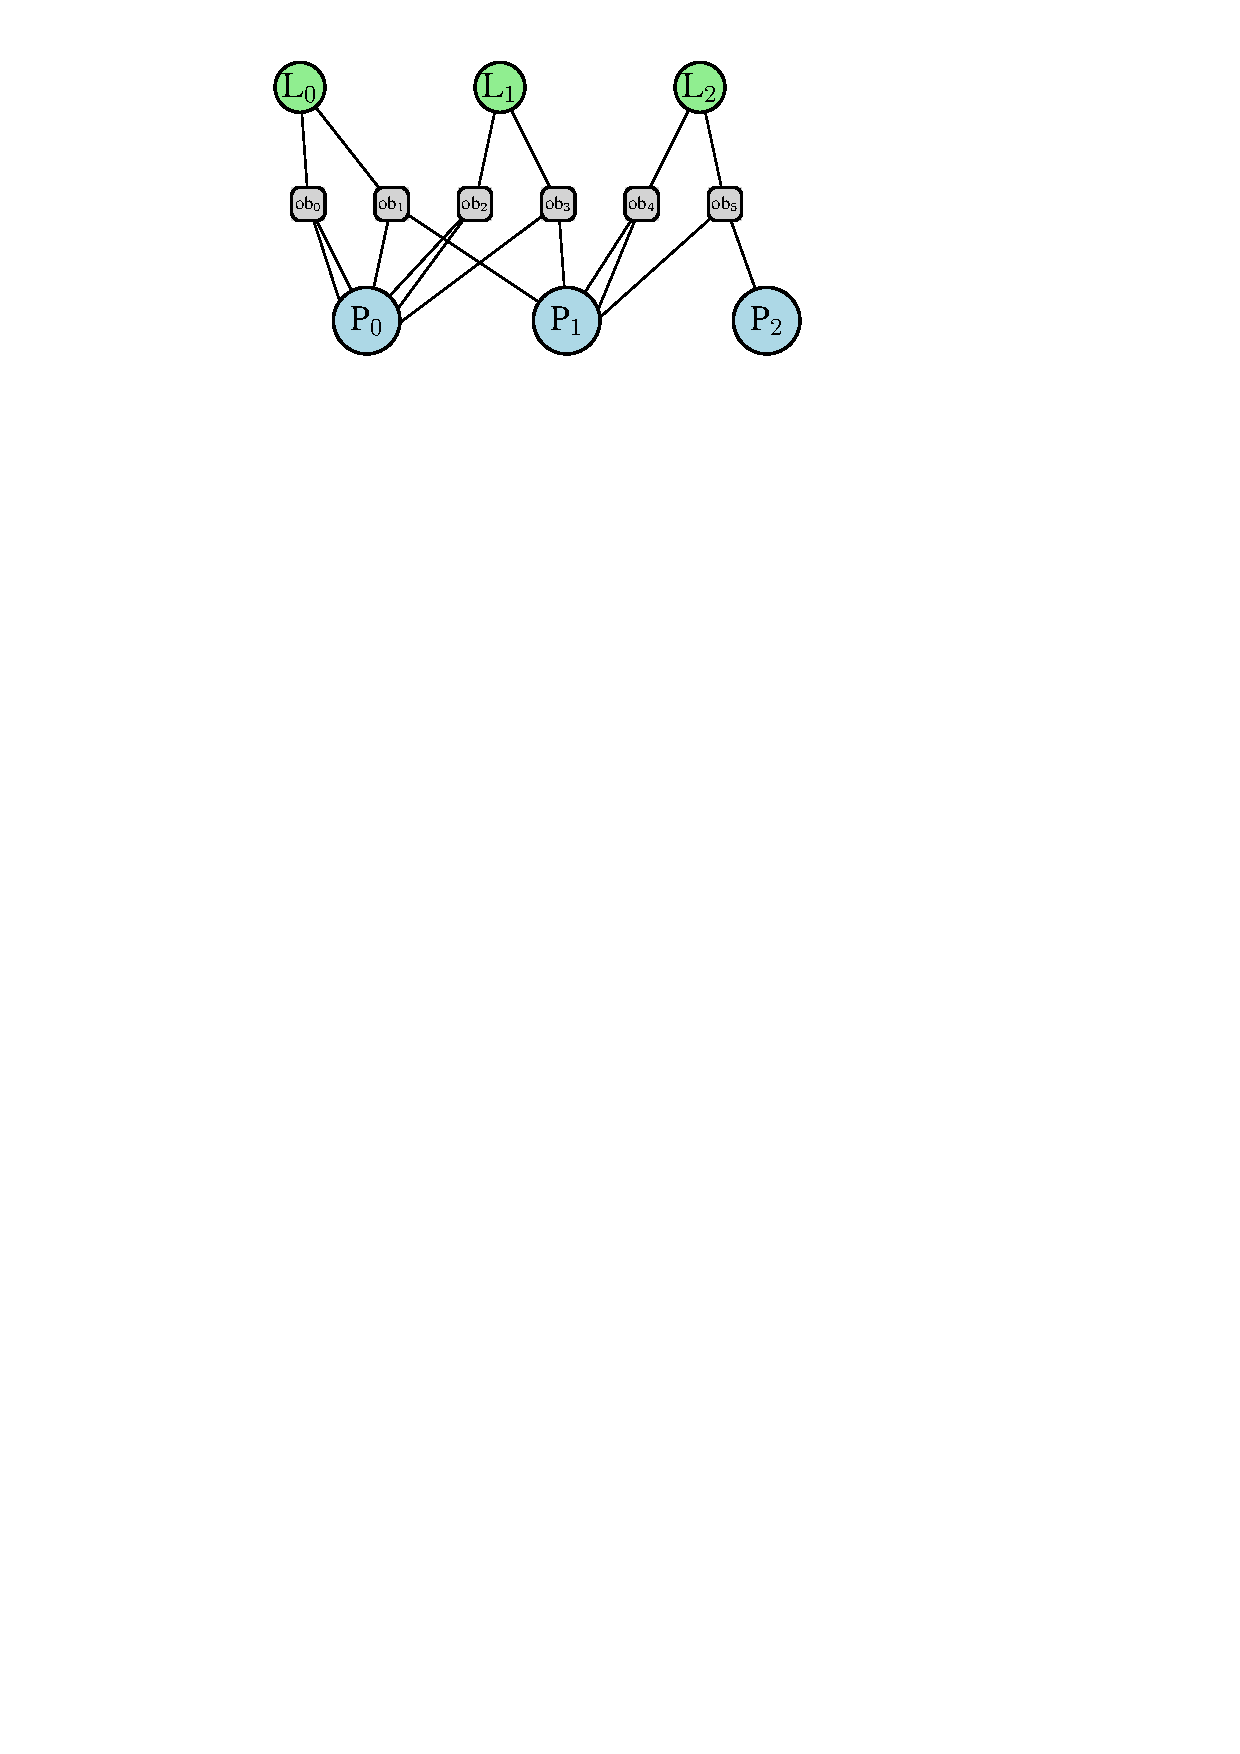
\includegraphics[width=0.5\textwidth]{chapters/images/inner_window}
  \caption{Inner window}
  \label{fig:inner_window}
\end{figure}

$\bv P_i$ represent 3D camera poses of keyframes and are therefore 6 dimensional (3 dimensions for translation, 3 for rotation).  $\bv L_i$ is a landmark position and is represented as a 3D vector in the frame of the keyframe where it was first recorded.  This will be referred to as the anchor keyframe.  It it important to note that the landmark is not represented in world coordinates, and therefore its position is also dependent on the anchor keyframe vertex state.

The edges which represent observations of landmarks are multi edges between the landmark, the anchor keyframe and the pose where it is observed from.  This also means the first observation of a landmark will contain two connections to the anchor keyframe.  The multi edge constraint is represented as a 3D vector - denoted as $\bv UVU$.  The first 2 values are the x and y pixel coordinates of the landmark as seen from the left frame of the stereo camera.  The third value is the x pixel coordinate in the right camera.  The reprojection error is calculated between the vertex states and multi edge as follows:

%TODO: FIX THIS NOTATION.  TERRIBLE TERRIBLE
\begin{align}
 \bv e = \bv{UVU} - map( ^{kf}\bv T_w \ ^w \bv T_{anchor} \ \bv L_{anchor}, \bv K )
\end{align}

$\bv L_{anchor}$ is the landmark in the anchor frame (landmark vertex).  $^w \bv T_{anchor}$ is the transform from the anchor keyframe to world frame (anchor keyframe vertex), and $^{kf}\bv T_w$ is the transformation from the world frame to the keyframe where this particular edge was recorded (observation keyframe).  The map function takes intrinsic camera calibration parameters and projects a 3D point into the pixel coordinates.

\subsection{Outer Window}

Unlike the bundle adjustment of the inner window, the outer window is a simple pose graph optimization.  It contains keyframe poses as in the inner window, and keyframe edges, which describe a transformation from one keyframe to another.  They are binary edges, only relating two poses at most.  The error function is then defined as follows:

%TODO: FIX THIS NOTATION.  TERRIBLE TERRIBLE
\begin{align}
 \bv e =  someLieGroupLogThing(^{w}\bv T_{kf_a} \ ^{kf_a} \bv T_{kf_b} \ ^{kf_b} \bv T_{w})
\end{align}

\begin{figure}[h!]
  \centering
    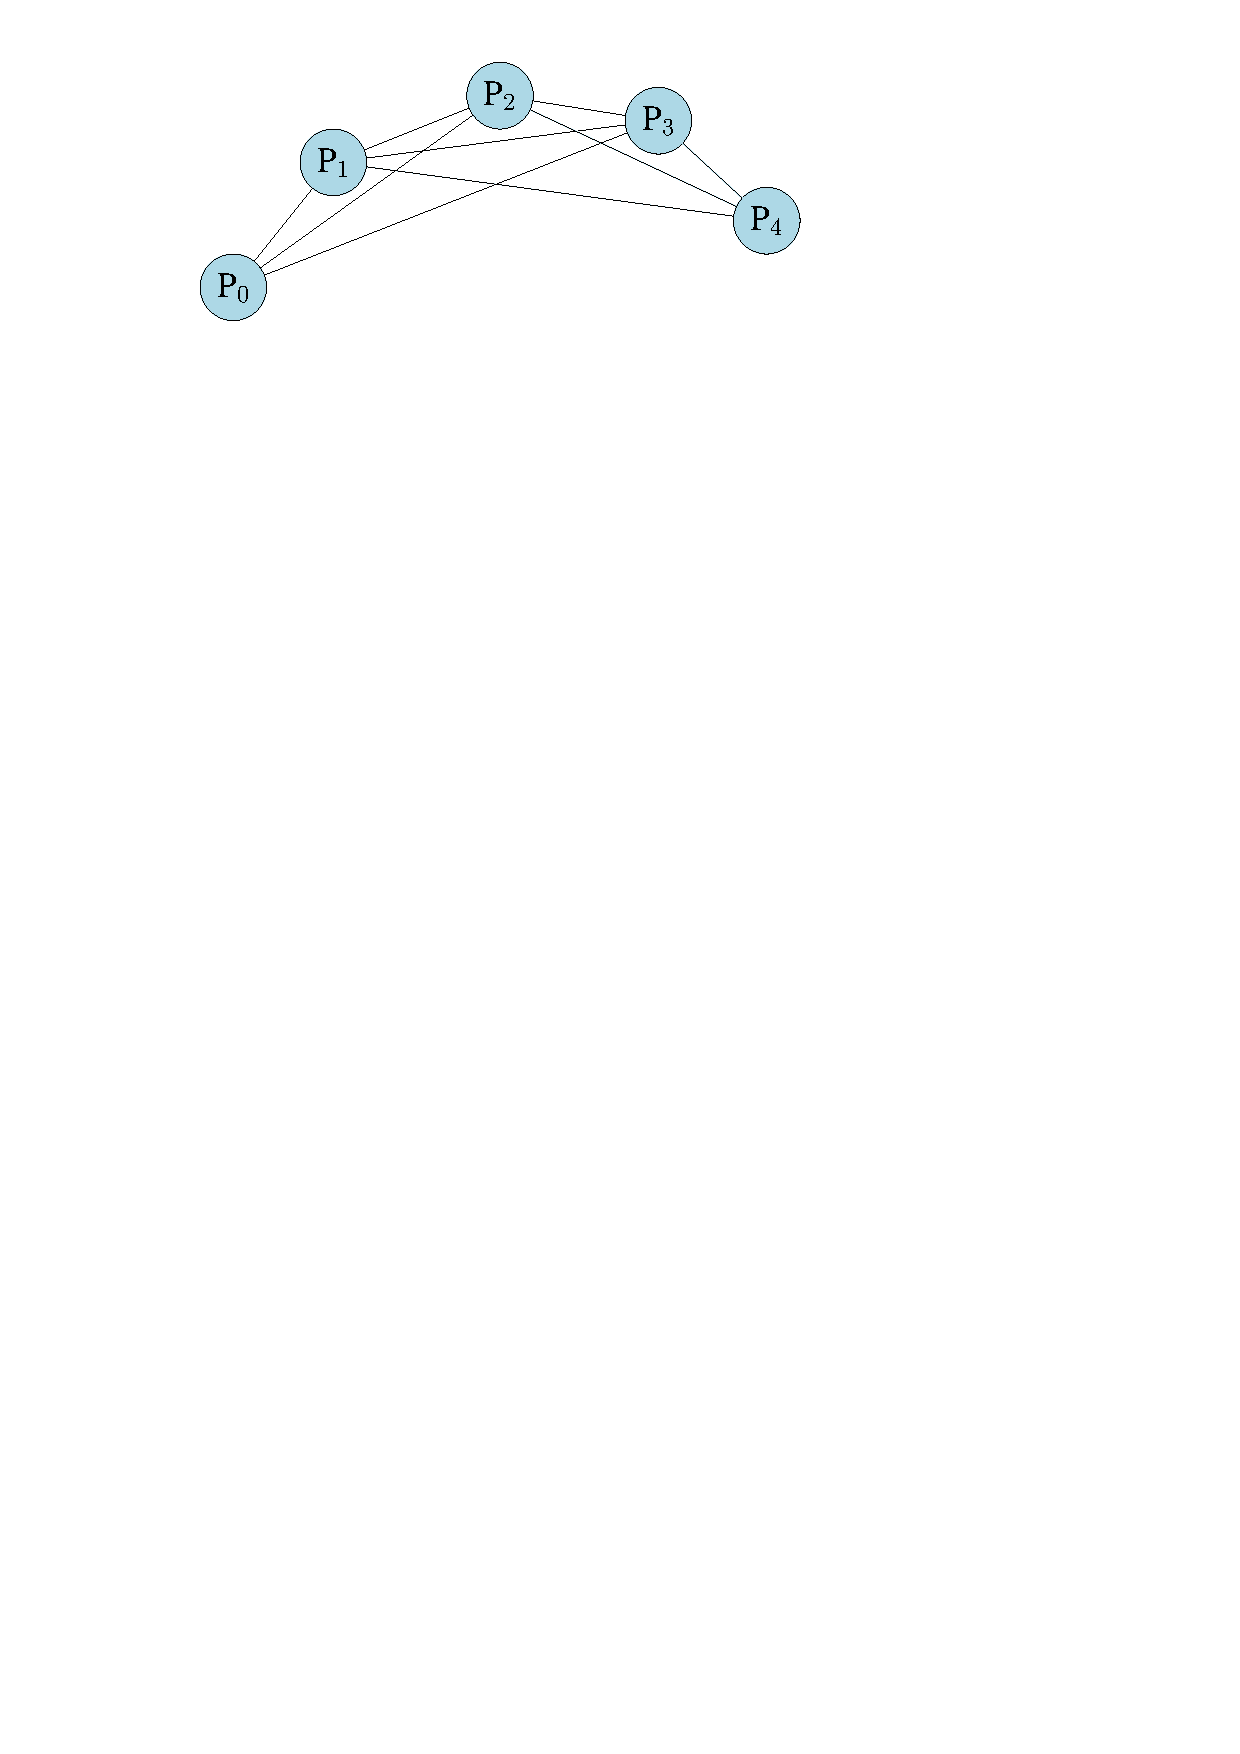
\includegraphics[width=0.5\textwidth]{chapters/images/outer_window}
  \caption{Outer window}
  \label{fig:outer_window}
\end{figure}

$^{w}\bv T_{kf_a}$ and $^{kf_b} \bv T_{w}$ are obtained from the vertex states, while $^{kf_a} \bv T_{kf_b}$ is the edge measurement.

\subsection{Window selection}


%\begin{itemize}
%\itemsep0em
 %\item SE(3) keyframes
 %\item SE(3) keyframe-keyframe edge
 %\item 3D Vector Landmark
 %\item 3D Vector UVU reprojection keyframe-landmark edge
%\end{itemize}
%
%\subsection{Double Window Graph Optimization}
%\begin{itemize}
%\itemsep0em
 %\item B.A. inner window
 %\item Pose-Pose outer window
 %\item metrics to define windows
 %\item ensures constant graph optimize time (novel from this approach)
%\end{itemize}
